\documentclass{article}
\usepackage[margin=2cm]{geometry}
\usepackage{listings}
\usepackage{float}
\usepackage{graphicx}

\lstset{basicstyle=\footnotesize, columns=fullflexible}

\setlength{\parskip}{10pt plus 1pt minus 1pt
\setlength{\parindent}{0cm}}

\begin{document}
\title{CS27020 Career Planner Assignment}
\author{Samuel Jackson \\ \texttt{slj11@aber.ac.uk}}
\date{\today}
\maketitle

\section{Introduction}
In this assignment, we have been tasked to design and create a single user database system to track a series of applications forms being made to a variety of different roles at different companies. For the basis of this assignment we were given an example application form with all the relevant data fields included.

Section two of this document deals with the design and normalization for the proposed database, while section three outlines the PostgreSQL database implementation of the design.

\section{Design}
This section details the design process that has been used to create the database system. Firstly the attributes required for each application are identified and outlined in un-normalized form. The functional dependencies for each attribute are then identified before proceeding through the stages of first, second and third normalization.

\subsection{Un-normalized Form and Functional Dependencies}
Using the application form document provided in the brief, the following structure for the database in its un-normalized form is as follows. I have also listed each of the repeating groups of attributes contained in the given un-normalized form.

\textbf{application}(company\_name, company\_info, role, deadline, req\_strength, req\_qualification, strength, evidence, satisfaction, qualification, date, grade, personal\_aim, relevance, CV, covering\_letter, date\_sent, response, interview\_date, outcome, reflection)

(req\_strength) Repeats for each required strength.\\
(req\_qualification) Repeats for each required qualification.\\
(strength, evidence, satisfaction) Repeats for each personal strength.\\
(qualification, date, grade) Repeats for each qualification.\\
(personal\_aim, relevance) Repeats for each personal aim.\\

Note that in the above outline I have shortened some of the attribute names to more concise abbreviations (e.g. Required Strength to ReqStrength).

\subsubsection{Assumptions}

In the above un-normalized form I have made several assumptions based on the document given by the brief to work from and of my own intuition. They are as follows:

The database is designed to handle the application forms of one user. In the brief there is no mention of the system having to handle any other users and therefore I have made the assumption that this database will only hold applications from one user at any one time.

Another assumption I have made is that, for each of the repeating attributes, the user may want to have more than simply three different entries as shown in the provided application form. I have therefore not considered any limit to these attributes and assume that each application can store an unspecified amount for each of these attributes.

I have also assumed that job applicant will only ever apply to the same role at the same company once. For example, my design cannot be used to apply to the same role at the same company but at another point in time. You could solve this problem by using the deadline for each application to further uniquely identify each application at a specific point in time. You could also accomplish the same result by adding an unique ID for each application.

One further assumption I have made is that there are never more than two roles with the same name in a company at the same time. Again, if this were not the case, we would probably have to look at including more attributes in the primary key, or adding a unique ID field to each record.

Another assumption I have made is that much of the documentation used for each application can be different. For example, the applicant may decide to send a different CV, covering letter or set of strengths/qualifications with each application depending on the role applied for.

\subsubsection{Functional Dependencies}
\label{sec:func}
Below are the functional dependencies for the un-normalized structure, including the repeating units. The majority of the attributes are dependant on the company name and role. This suggests that company name and role are a composite key and are an excellent candidate for the primary key. This is because all of the data applied for can be uniquely identified by the name of the company and the role applied for within that company. 

Note that we cannot simply use just a the company name or just the role to uniquely identify a data because a company may have many roles and the same role may be offered by many companies. Therefore the primary key must be a composite key consisting of both attributes. 

Alternative keys could include a large composite key, such as including the deadline to specify which point in time the role was offered, solving the problem with the same company offering the same role in the future, but as I have stated in my assumptions, I believe this system is only designed to by used by one user at one point in time without having to consider the same role being offered twice. Therefore be using a composite key consisting of the company name and the role as my primary key for this design.

(company\_name, role) $\rightarrow$ \{company\_info, deadline, req\_strength, req\_qualifications, strength, qualification, personal\_aim, CV, covering\_letter, date\_sent, response, interview\_date, outcome, feedback, reflection\}

company\_name $\rightarrow$ \{company\_info\}\\
strength $\rightarrow$ \{evidence, satisfaction\}\\
qualification $\rightarrow$ \{date, grade\}\\
personal\_aim $\rightarrow$ \{relevance\}\\

Working through the functional dependencies in turn, we can see that the company name and role advertised is enough to determine when the application deadline is, the various requirements for the role (Qualifications, Strengths etc.) as well as the documentation that is required for it, such as a CV and covering letter. 

Information about the company is obviously dependant on the name of the company and therefore does not require information of the role to determine it.

The attributes evidence and satisfaction can be determined by the just the name of the personal strength as the evidence and satisfaction given by the strength is obviously dependant on what the strength actually is.

Similarly, the attributes of date and grade are dependant on what the qualification actually is.

Finally the relevance of a personal aim can again only be determined once you know what the aim actually is and therefore the relevance of an aim relies of the individual aim alone.

\subsection{First Normal Form}

Once we identified the primary key to be used and the functional dependencies of the system, we can start normalising the structure. In first normal form we remove any repeating units from the main relation and put them in their own separate relation. Bringing the un-normalized structure given in the previous section to first normal form gives the following relations:

\textbf{application}(\underline{company\_name}, \underline{role}, company\_info, deadline, CV, covering\_letter, date\_sent, response, interview\_date, outcome, feedback, reflection)

\textbf{req\_strengths}(\underline{strength}, \underline{company\_name}*, \underline{role}*)

\textbf{req\_qualifications}(\underline{qualification}, \underline{company\_name}*, \underline{role}*)

\textbf{strengths}(\underline{strength}, \underline{company\_name}*, \underline{role}*, evidence, satisfaction)

\textbf{qualifications}(\underline{qualification}, \underline{company\_name}*, \underline{role}*, date, grade)

\textbf{aims}(\underline{personal\_aim}, \underline{company\_name}*, \underline{role}*, relevance)

In the above scheme I have removed all repeating units found in the un-normalized form along with any attributes that are functionally dependent on them from the application relation and made them into separate relation. This reduces the repetition and redundancy of data across the system. Note that I have also moved the required strengths and qualifications from the application relation as these are also repeating attributes, despite not having any other attributes being functionally dependant on them.

\subsection{Second \& Third Normal Form}

In second normal form we must ensure that every attribute in a relation is fully functionally dependant on the primary key. This means that any attribute that is only partially dependant on the primary key for that relation must be split into a smaller relation that removes the partial dependency. By rearranging the relations specified in the preceding section we get the following structure:

\textbf{application}(\underline{company\_name}*, \underline{role}, deadline, CV, covering\_letter, date\_sent, response, interview\_date, outcome, feedback, reflection)

\textbf{company}(\underline{name}, information)

\textbf{strength\_link}(\underline{strength}*, \underline{company\_name}*, \underline{role}*)

\textbf{qualification\_link}(\underline{qualification}*, \underline{company\_name}*, \underline{role}*)

\textbf{strengths}(\underline{strength}, evidence, satisfaction)

\textbf{qualifications}(\underline{qualification}, date, grade)

\textbf{req\_strengths}(\underline{strength}, \underline{company\_name}*, \underline{role}*)

\textbf{req\_qualifications}(\underline{qualification}, \underline{company\_name}*, \underline{role}*)

\textbf{aims}(\underline{personal\_aim}, \underline{company\_name}*, \underline{role}*, relevance)

Company name and company information can be moved from the application relation at this stage because it is only partially functionally dependant on the primary key (specifically the company name). This also correlates with the functional dependencies outlined in section \ref{sec:func}. Therefore we can move this to its own relation.

Similarly, we must move both the strengths and qualifications to their own relations as the evidence and satisfaction only depend on the strength and the date and grade only depend on the qualification. None of these attributes depend on the company name or role, and therefore are only partially dependant on there primary key in first normal form. I have also created a linking table for each of them to organise what strengths and qualifications are related to a particular application.

Both required strengths and required qualifications need to be adjusted at this stage because neither required strength or required qualification is partially dependant on the composite key of company and role. 

Likewise, the aims relation does not need to be changed as the relevance of a personal aims depends on the company name, the role and the personal aim itself because the relevance of an aim may change between roles, and companies (e.g. learning python might not be a good aim for a job that specifies it needs a Java programmer, but it is an excellent aim for a python developer).

Since we have removed all partial dependencies from the relational structure the database design is now in second normal form. It is also the case that the steps taken in this section have removed any transitive dependencies that may have existed in first normal form, and therefore this structure in now automatically in third normal form.

\section{Implementation}
\subsection{Database Creation}
In this section I provide a full typescript copy of the SQL statements that were executed on the database in order to created the tables and relations required.

% Following line imports the database creation script
\lstinputlisting[language=sql, caption=PostgreSQL statements used to create the database]{sql/create.sql}

Below I provide two screenshots showing the the execution of the preceding script on the university database and a listing of the created tables:

%include screen shots of database creation
\begin{figure}[H]
\centering
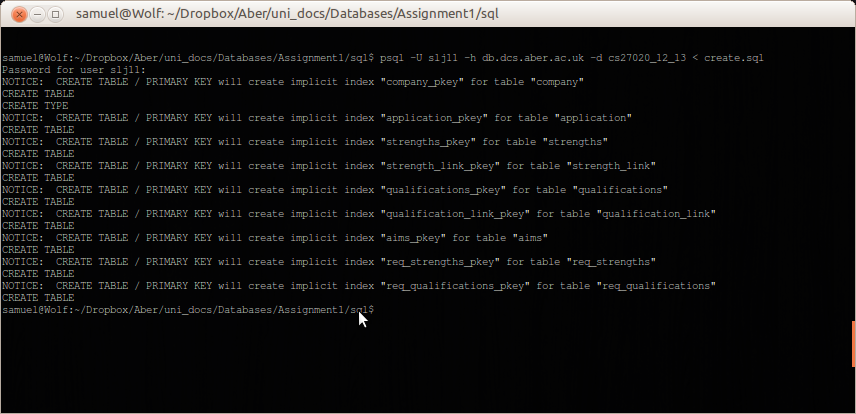
\includegraphics[width=0.7\textwidth]{img/db-create.png}
\caption{Executing the database creation script on the database}
\label{fig:db-create}
\end{figure}

\begin{figure}[H]
\centering
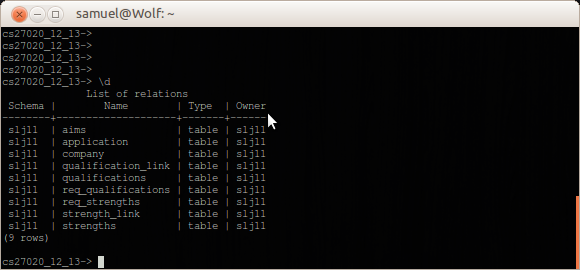
\includegraphics[width=0.7\textwidth]{img/db-show-tables.png}
\caption{The resulting tables created after the scripts execution}
\label{fig:db-show-tables}
\end{figure}

\subsubsection{Justification of Data Types}
In my database structure, I have used a variety of different types to create the fields used in my database. Here I provide justification of my choices of data types for each attribute used. Where there are two or more attributes representing the same thing in different tables (e.g. part of a foreign key) I will not justify there data type as they are already specified elsewhere.

\begin{itemize}
\item \textbf{varchar} - I have used the varchar data type for fields in my design where I can potentially limit the number of characters required to a reasonable number. Examples of this include company name, strength, required strength, qualification, required qualification. This is because it can be assumed that each of these attributes can be described in (or abbreviated to) less than 50 characters. There are a couple of exceptions to the 50 character limit discussed below:

\begin{itemize}
\item Attributes such as the personal\_aim and relevance of aims and the evidence and satisfaction of strengths have been set to have a character limit of 500. This is because even though it is not certain how large the data in these fields are likely to be, I feel 500 characters is a reasonable amount of space.

\item The grade of a qualification has a character limit of 3. This is so that the field can store both letter grades such as A++, B or C- as well as being able to store degree level qualification grades such as 1:1, 2:1, 2:2 etc. 

\item Attributes relating to large data fields that are supposedly going to contain URL links rather than actual data (such as CV and company information), have been set to be a varchar with the length of 2000 characters. This is because web browsers such as IE do not support URL lengths much above this limit.\footnote{http://support.microsoft.com/kb/208427}

\end{itemize}

\item \textbf{date} - The date data type is used wherever an attribute is storing data related to a specific date. Date was chosen over other data types such as timestamp, because only knowledge of the date is required and I am assuming that there is no information regarding specific times that need to be stored. Example fields that use this in the database are qualification\_date, interview\_date and deadline.

\item \textbf{result} - This is a custom enumeration that I have created to represent the state of the application's outcome. The possible values are:

\begin{itemize}
	\item ACCEPTED - If the application was successful.
	\item REJECTED - If the application failed.
	\item N/A - If the application is pending and has not been accepted or rejected. The outcome field will take this value by default.
\end{itemize}

I decided to use an enumeration for this value because I felt this was the simplest way to represent three distinct states that the application can be in. It also leaves the design open for extension, as more states can easily be added in the future (such as a state for pending interview or pending response etc.)

\end{itemize}

\subsection{Testing the Database}
In order to thoroughly test the database, I created a selection of queries to input and retrieve data from the system. I have also created a selection of erroneous queries to demonstrate the constraints placed in effect the attributes.

\subsubsection{Testing with Erroneous Queries}
The first query I created demonstrates the primary key constraint that I have used to restrict the company name to be not null and unique. I have used the same technique multiple times across the implementation. When a record is inserted that has a primary key that already exists, the database with throw an error. And example of this is shown below:

\begin{figure}[H]
\centering
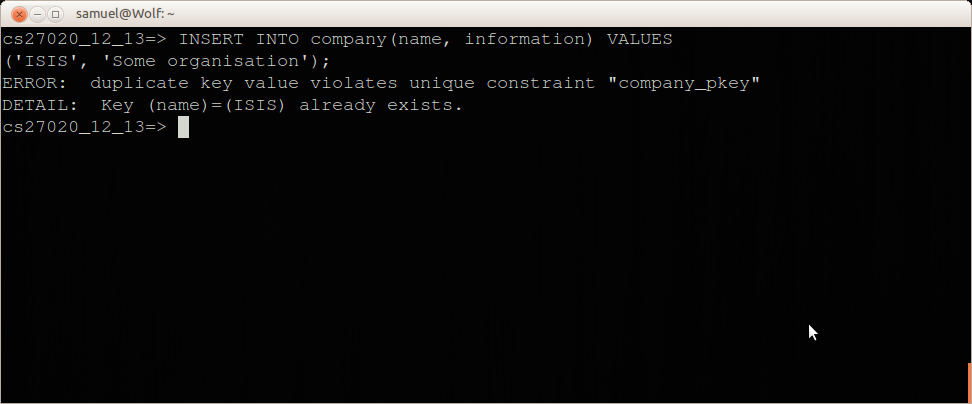
\includegraphics[width=0.7\textwidth]{img/test/test-pkey.png}
\caption{Attempting to create a record with a primary key that already exists}
\label{fig:test-pkey}
\end{figure}

Primary key constraints also force the user to always specify a primary key, the following example fails because it leaves of the non-optional primary key field.

\begin{figure}[H]
\centering
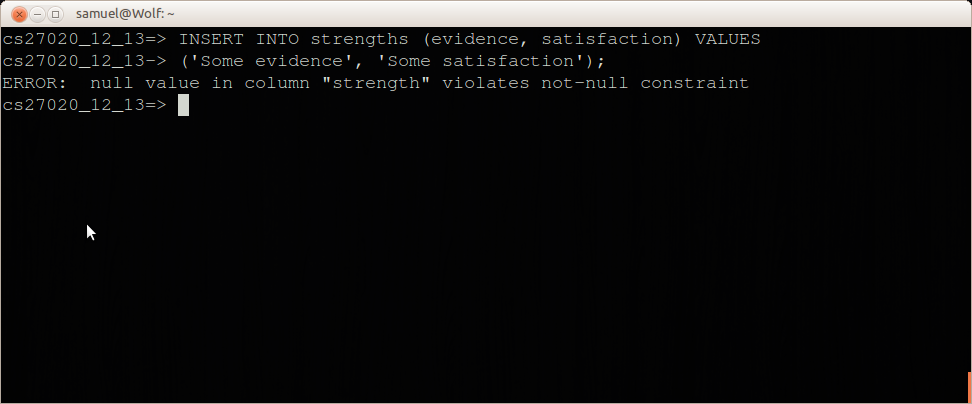
\includegraphics[width=0.7\textwidth]{img/test/test-pkey-empty.png}
\caption{Attempting to create a record where the primary key is empty}
\label{fig:test-pkey-empty}
\end{figure}

The next query that I have created demonstrates the use of a foreign key constraint on the application's table. Like the use of the primary key constraint, I have used the foreign key constraint across the design to ensure that data is correctly referenced from the right relation and that a record with a foreign key that does not exist is not inserted. Below is an example of this:

\begin{figure}[H]
\centering
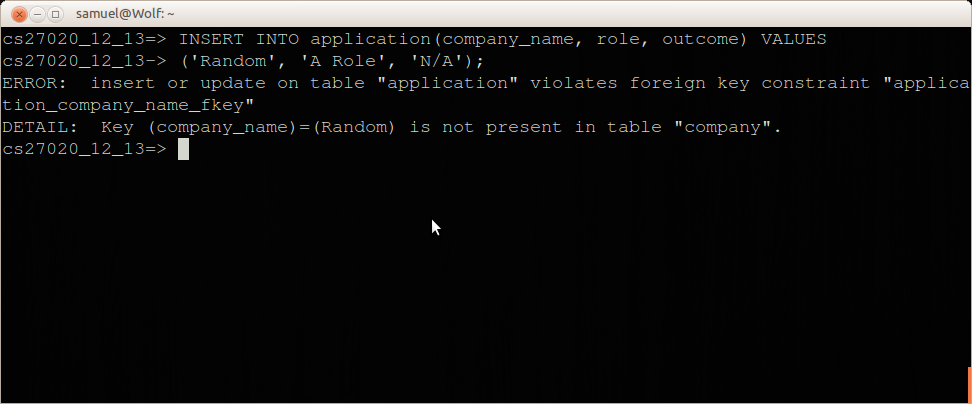
\includegraphics[width=0.7\textwidth]{img/test/test-fkey.png}
\caption{Testing the database with a foreign key that does not exist}
\label{fig:test-fkey}
\end{figure}

This behaviour can be used to prevent a linking table from connecting a strength or qualification that does not exist to an application, as shown in the following screenshot:

\begin{figure}[H]
\centering
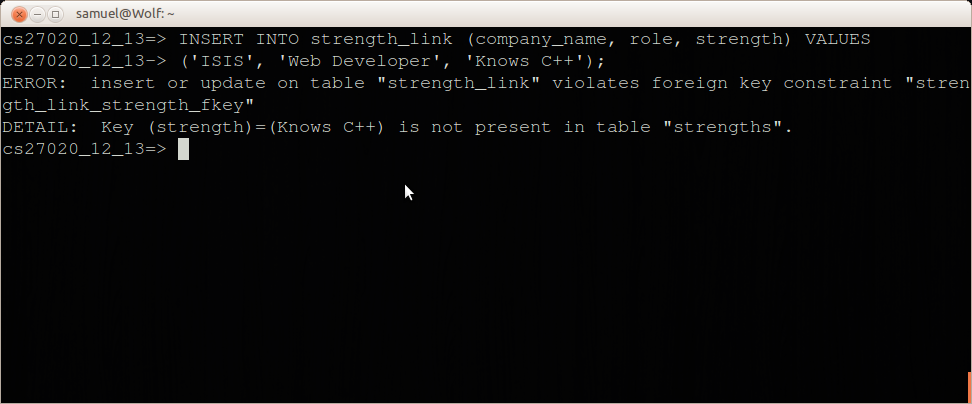
\includegraphics[width=0.7\textwidth]{img/test/test-fkey-link.png}
\caption{Testing attempting to link a non existent foreign field to an application.}
\label{fig:test-fkey-link}
\end{figure}

Another query shows an example of the type constraints that I have used as part of my design. Many fields require a specific type of data, such as a date. Setting the attribute to only accept data in the format of a date ensures the database only accepts correctly formatted input. An example of this is shown below:

\begin{figure}[H]
\centering
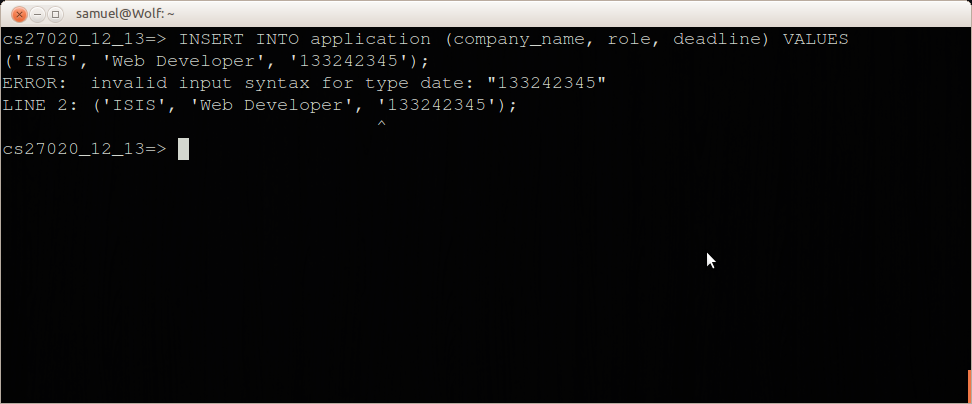
\includegraphics[width=0.7\textwidth]{img/test/test-date.png}
\caption{Testing the date type constraint}
\label{fig:test-date}
\end{figure}


\end{document}
